% Options for packages loaded elsewhere
\PassOptionsToPackage{unicode}{hyperref}
\PassOptionsToPackage{hyphens}{url}
%
\documentclass[
  ignorenonframetext,
  aspectratio=43,
]{beamer}
\usepackage{pgfpages}
\setbeamertemplate{caption}[numbered]
\setbeamertemplate{caption label separator}{: }
\setbeamercolor{caption name}{fg=normal text.fg}
\beamertemplatenavigationsymbolshorizontal
% Prevent slide breaks in the middle of a paragraph
\widowpenalties 1 10000
\raggedbottom
\setbeamertemplate{part page}{
  \centering
  \begin{beamercolorbox}[sep=16pt,center]{part title}
    \usebeamerfont{part title}\insertpart\par
  \end{beamercolorbox}
}
\setbeamertemplate{section page}{
  \centering
  \begin{beamercolorbox}[sep=12pt,center]{part title}
    \usebeamerfont{section title}\insertsection\par
  \end{beamercolorbox}
}
\setbeamertemplate{subsection page}{
  \centering
  \begin{beamercolorbox}[sep=8pt,center]{part title}
    \usebeamerfont{subsection title}\insertsubsection\par
  \end{beamercolorbox}
}
\AtBeginPart{
  \frame{\partpage}
}
\AtBeginSection{
  \ifbibliography
  \else
    \frame{\sectionpage}
  \fi
}
\AtBeginSubsection{
  \frame{\subsectionpage}
}

\usepackage{amsmath,amssymb}
\usepackage{lmodern}
\usepackage{iftex}
\ifPDFTeX
  \usepackage[T1]{fontenc}
  \usepackage[utf8]{inputenc}
  \usepackage{textcomp} % provide euro and other symbols
\else % if luatex or xetex
  \usepackage{unicode-math}
  \defaultfontfeatures{Scale=MatchLowercase}
  \defaultfontfeatures[\rmfamily]{Ligatures=TeX,Scale=1}
\fi
\usetheme[]{default}
\usecolortheme{default}
% Use upquote if available, for straight quotes in verbatim environments
\IfFileExists{upquote.sty}{\usepackage{upquote}}{}
\IfFileExists{microtype.sty}{% use microtype if available
  \usepackage[]{microtype}
  \UseMicrotypeSet[protrusion]{basicmath} % disable protrusion for tt fonts
}{}
\makeatletter
\@ifundefined{KOMAClassName}{% if non-KOMA class
  \IfFileExists{parskip.sty}{%
    \usepackage{parskip}
  }{% else
    \setlength{\parindent}{0pt}
    \setlength{\parskip}{6pt plus 2pt minus 1pt}}
}{% if KOMA class
  \KOMAoptions{parskip=half}}
\makeatother
\usepackage{xcolor}
\newif\ifbibliography
\setlength{\emergencystretch}{3em} % prevent overfull lines
\setcounter{secnumdepth}{-\maxdimen} % remove section numbering


\providecommand{\tightlist}{%
  \setlength{\itemsep}{0pt}\setlength{\parskip}{0pt}}\usepackage{longtable,booktabs,array}
\usepackage{calc} % for calculating minipage widths
\usepackage{caption}
% Make caption package work with longtable
\makeatletter
\def\fnum@table{\tablename~\thetable}
\makeatother
\usepackage{graphicx}
\makeatletter
\def\maxwidth{\ifdim\Gin@nat@width>\linewidth\linewidth\else\Gin@nat@width\fi}
\def\maxheight{\ifdim\Gin@nat@height>\textheight\textheight\else\Gin@nat@height\fi}
\makeatother
% Scale images if necessary, so that they will not overflow the page
% margins by default, and it is still possible to overwrite the defaults
% using explicit options in \includegraphics[width, height, ...]{}
\setkeys{Gin}{width=\maxwidth,height=\maxheight,keepaspectratio}
% Set default figure placement to htbp
\makeatletter
\def\fps@figure{htbp}
\makeatother

\usepackage{ragged2e}
\usepackage{etoolbox}

\apptocmd{\frame}{}{\justifying}{} 

\setbeamertemplate{enumerate items}[default]
\setbeamertemplate{itemize items}[circle]
\setbeamersize{text margin left=2.25em, text margin right=2.25em}

\let\OLDitemize\itemize
\renewcommand\itemize{
    \OLDitemize\addtolength{\itemsep}{3pt plus 1pt minus 1pt}
}
\let\OLDenumerate\enumerate
\renewcommand\enumerate{
    \OLDenumerate\addtolength{\itemsep}{3pt plus 1pt minus 1pt}
}

\usepackage{orcidlink}
\usepackage{amsmath}
\DeclareMathOperator*{\argmax}{argmax}

\makeatletter
\def\@listii{\leftmargin\leftmarginii
              \topsep    1ex
              \parsep    0\p@   \@plus\p@
              \itemsep   \parsep}
\makeatother

\usepackage{lipsum}

\let\olditem\item
\renewcommand\item{\olditem\justifying}

\definecolor{blue}{RGB}{0,114,178}
\definecolor{red}{RGB}{213,94,0}
\definecolor{yellow}{RGB}{240,228,66}
\definecolor{green}{RGB}{0,158,115}

\definecolor{MyBackground}{RGB}{255,253,218}

\setbeamercolor{section in toc}{fg=blue}
\setbeamercolor{subsection in toc}{fg=red}

\setbeamercolor{frametitle}{fg=blue}
\setbeamercolor{title}{fg=blue}

\setbeamertemplate{footline}[frame number]
\setbeamertemplate{navigation symbols}{} 
\setbeamertemplate{itemize items}{-}

\setbeamercolor{itemize item}{fg=blue}
\setbeamercolor{itemize subitem}{fg=blue}
\setbeamercolor{enumerate item}{fg=blue}
\setbeamercolor{enumerate subitem}{fg=blue}
\setbeamercolor{button}{bg=MyBackground,fg=blue}

\newcounter{daggerfootnote}
\newcommand*{\daggerfootnote}[1]{%
    \setcounter{daggerfootnote}{\value{footnote}}%
    \renewcommand*{\thefootnote}{\fnsymbol{footnote}}%
    \footnote[2]{#1}%
    \setcounter{footnote}{\value{daggerfootnote}}%
    \renewcommand*{\thefootnote}{\arabic{footnote}}%
}

\AtBeginSection{
    \begingroup
    \setbeamercolor{background canvas}{bg=yellow}
    \begin{frame}
        \begin{centering}
            \usebeamerfont{section title}\huge\color{black}\insertsection\par
        \end{centering}
    \end{frame}
    \endgroup
}
\makeatletter
\makeatother
\makeatletter
\makeatother
\makeatletter
\@ifpackageloaded{caption}{}{\usepackage{caption}}
\AtBeginDocument{%
\ifdefined\contentsname
  \renewcommand*\contentsname{Table of contents}
\else
  \newcommand\contentsname{Table of contents}
\fi
\ifdefined\listfigurename
  \renewcommand*\listfigurename{List of Figures}
\else
  \newcommand\listfigurename{List of Figures}
\fi
\ifdefined\listtablename
  \renewcommand*\listtablename{List of Tables}
\else
  \newcommand\listtablename{List of Tables}
\fi
\ifdefined\figurename
  \renewcommand*\figurename{Figure}
\else
  \newcommand\figurename{Figure}
\fi
\ifdefined\tablename
  \renewcommand*\tablename{Table}
\else
  \newcommand\tablename{Table}
\fi
}
\@ifpackageloaded{float}{}{\usepackage{float}}
\floatstyle{ruled}
\@ifundefined{c@chapter}{\newfloat{codelisting}{h}{lop}}{\newfloat{codelisting}{h}{lop}[chapter]}
\floatname{codelisting}{Listing}
\newcommand*\listoflistings{\listof{codelisting}{List of Listings}}
\makeatother
\makeatletter
\@ifpackageloaded{caption}{}{\usepackage{caption}}
\@ifpackageloaded{subcaption}{}{\usepackage{subcaption}}
\makeatother
\makeatletter
\@ifpackageloaded{tcolorbox}{}{\usepackage[many]{tcolorbox}}
\makeatother
\makeatletter
\@ifundefined{shadecolor}{\definecolor{shadecolor}{rgb}{.97, .97, .97}}
\makeatother
\makeatletter
\makeatother
\ifLuaTeX
  \usepackage{selnolig}  % disable illegal ligatures
\fi
\IfFileExists{bookmark.sty}{\usepackage{bookmark}}{\usepackage{hyperref}}
\IfFileExists{xurl.sty}{\usepackage{xurl}}{} % add URL line breaks if available
\urlstyle{same} % disable monospaced font for URLs
\hypersetup{
  pdftitle={Seminar 4},
  pdfauthor={Gabriel E. Cabrera Guzmán},
  hidelinks,
  pdfcreator={LaTeX via pandoc}}

\title[Seminar 4]{Seminar
4\daggerfootnote{\texttt{gabriel.cabreraguzman@postgrad.manchester.ac.uk}}}
\subtitle{Probability 3 \& 4 (Normal, Binomial, Poisson \& Exponential
Distributions) Solutions}
\author[Gabriel E. Cabrera Guzmán]{
    {Gabriel E. Cabrera
Guzmán\textsuperscript{\normalsize\orcidlink{0000-0000-0000-0000}}} \medskip
}
\date{October 31, 2025}
\institute[]{
    The University of Manchester\\
Alliance Manchester Business School \bigskip
}

\definecolor{quarto-callout-note-color}{RGB}{0,114,178}
\definecolor{quarto-callout-note-color-frame}{RGB}{0,114,178}
\definecolor{quarto-callout-warning-color}{RGB}{213,94,0}
\definecolor{quarto-callout-warning-color-frame}{RGB}{213,94,0}
\begin{document}
\frame{\titlepage}
\ifdefined\Shaded\renewenvironment{Shaded}{\begin{tcolorbox}[boxrule=0pt, interior hidden, borderline west={3pt}{0pt}{shadecolor}, sharp corners, enhanced, breakable, frame hidden]}{\end{tcolorbox}}\fi

\begin{frame}{Exercise 1}
\protect\hypertarget{exercise-1}{}
A financial analyst predicts that the return on Whizzco ordinary shares
over the next 12-month period is equally likely to be any percentage
between -2\% and 4\%. Assuming that the analyst is correct:

\begin{enumerate}
\item
  Draw the probability density function (PDF) of the return, X, and
  write down its formula f(x).

  \pause

  \textbf{A:} This is a uniform distribution for a random variable
  \(-2 = a \le X \le b = 4\), with the following probability density
  function (PDF):

  \[
  f(x) = \frac{1}{b - a} = \frac{1}{4 - (-2)} = \frac{1}{6}
  \]
\end{enumerate}
\end{frame}

\begin{frame}{Exercise 1 (Cont'd)}
\protect\hypertarget{exercise-1-contd}{}
\begin{enumerate}
\setcounter{enumi}{1}
\item
  Calculate the probability that the share has a positive return.

  \pause

  \textbf{A:} The probability that the return is positive (\(X \ge 0\))
  is: \vspace{-4pt}

  \[
  \Pr(X \ge 0) = \text{length} \times \text{width} = 4 \times \frac{1}{6} = \frac{2}{3}
  \]
\item
  Write down the mean and variance of the share's return.

  \pause

  \textbf{A:} The mean of the uniform distribution is
  \(\frac{a + b}{2}\), and the variance is
  \(\sigma^2 = \frac{(b - a)^2}{12}\). Thus,

  \(\text{Mean} = \frac{(-2) + 4}{2} = 1\) and
  \(\text{Variance} = \frac{(4 - (-2))^2}{12} = \frac{6^2}{12} = 3\)
\end{enumerate}
\end{frame}

\begin{frame}{Exercise 2}
\protect\hypertarget{exercise-2}{}
When Z is a standard normal random variable Pr(Z \textless{} -1.5) =
0.0668. Deduce the following without using tables.

\begin{enumerate}
\item
  \(\Pr(Z > -1.5)\)

  \pause

  \textbf{A}: We know that \(Z\) is a standard normal random variable
  and \(\Pr(Z < -1.5) = 0.0668\). Hence: \vspace{-15pt}

  \[
  \Pr(Z > -1.5) = 1 - \Pr(Z < -1.5) = 1 - 0.0668 = 0.9332
  \]
\item
  \(\Pr(Z > 1.5)\)

  \pause

  \textbf{A}: \vspace{-15pt}

  \[  
  \Pr(Z > 1.5) = \Pr(Z < -1.5) = 0.0668
  \]
\end{enumerate}
\end{frame}

\begin{frame}{Exercise 2 (Cont'd)}
\protect\hypertarget{exercise-2-contd}{}
\begin{enumerate}
\setcounter{enumi}{2}
\item
  \(\Pr(-1.5 < Z < 1.5)\)

  \pause

  \textbf{A}: \vspace{-15pt}

  \[
  \begin{aligned}
  \Pr(-1.5 < Z < 1.5) &= 1 - 2 \Pr(Z < -1.5) \\ 
                      &= 1 - 2(0.0668) = 0.8664
  \end{aligned}
  \]
\item
  \(\Pr(|Z| > 1.5)\)

  \pause

  \textbf{A}: \vspace{-20pt}

  \[
  \Pr(|Z| > 1.5) = 2 \Pr(Z < -1.5) = 2(0.0668) = 0.1336
  \]
\end{enumerate}
\end{frame}

\begin{frame}{Exercise 3}
\protect\hypertarget{exercise-3}{}
Calculate the following assuming that \(X \sim N(100,64)\).

\begin{enumerate}
\item
  \(\Pr(X > 120)\)

  \pause

  \textbf{A}:

  Because \(X \sim N(100, 64)\), the random variable \(X\) is normal,
  with mean \(\mu = 100\) and variance \(\sigma^2 = 64\) (i.e., standard
  deviation \(\sigma = 8\)). Hence:

  \[
  \begin{aligned}
  \Pr(X > 120) 
  &= \Pr\left( \frac{X - 100}{8} > \frac{120 - 100}{8} \right) \\
  &= \Pr(Z > 2.5) \\
  &= 1 - \Pr(Z < 2.5) \\ 
  &= 1 - 0.9938 \\
  &= 0.0062 \\
  \end{aligned}
  \]
\end{enumerate}
\end{frame}

\begin{frame}{Exercise 3 (Cont'd)}
\protect\hypertarget{exercise-3-contd}{}
\begin{enumerate}
\setcounter{enumi}{1}
\item
  \(\Pr(X \leq 99)\)

  \pause

  \textbf{A}: \vspace{-20pt}

  \[
  \Pr(X \le 99) 
  = \Pr\left( \frac{X - 100}{8} \le \frac{99 - 100}{8} \right) 
  = \Pr(Z \le -0.125)
  \]

  By symmetry,
  \(\Pr(Z \le -0.125) = \Pr(Z \ge 0.125) = 1 - \Pr(Z < 0.125)\). Using
  interpolation between 0.5478 and 0.5517:

  \[
  \Pr(Z < 0.125) = \frac{0.5478 + 0.5517}{2} = 0.54975
  \]

  Thus,

  \[
  \Pr(X \le 99) = 1 - 0.54975 = 0.45025
  \]
\end{enumerate}
\end{frame}

\begin{frame}{Exercise 3 (Cont'd)}
\protect\hypertarget{exercise-3-contd-1}{}
\begin{enumerate}
\setcounter{enumi}{2}
\item
  \(\Pr(90< X < 100)\)

  \pause

  \textbf{A}: \vspace{-20pt}

  \[
  \begin{aligned}
  \Pr(90 < X < 100) 
  &= \Pr\left( \frac{90 - 100}{8} < \frac{X - 100}{8} < \frac{100 - 100}{8} \right) \\
  &= \Pr(-1.25 < Z < 0)
  \end{aligned}
  \]

  \[
  \begin{aligned}
  \Pr(-1.25 < Z < 0) &= \Pr(0 < Z < 1.25) \\
  &= \Pr(Z < 1.25) - \Pr(Z < 0) \\
  &= 0.8944 - 0.5 = 0.3944
  \end{aligned}
  \]
\end{enumerate}
\end{frame}

\begin{frame}{Exercise 4}
\protect\hypertarget{exercise-4}{}
X has a normal distribution with a mean of \(\mu=4\) and a standard
deviation of \(\sigma=1.5\). Find the critical value a such that
\(Pr(4-a < X < 4+a) = 0.8\).

\pause

\textbf{A}: This question asks us to find the range for a random
variable, given a certain level of confidence (i.e., probability or area
under the curve). Indeed, we need to find \(a\) such that \vspace{-7pt}

\[
\Pr(4 - a < X < 4 + a) = 0.8
\]

First, standardize the random variable \(X\):

\[
\begin{aligned}
\Pr\left( \frac{4 - a - 4}{1.5} < \frac{X - 4}{1.5} < \frac{4 + a - 4}{1.5} \right) 
&= 0.8 \\
\Pr\left( \frac{-a}{1.5} < Z < \frac{a}{1.5} \right) &= 0.8
\end{aligned}
\]
\end{frame}

\begin{frame}{Exercise 4 (Cont'd)}
\protect\hypertarget{exercise-4-contd}{}
Define \(\frac{a}{1.5} = b\). Hence, we have \(\Pr(-b < Z < b) = 0.8\).
What is the value of \(b\) on the horizontal axis such that the area
under the standard normal distribution between \(-b\) and \(b\) is equal
to 0.8?

\begin{figure}

{\centering 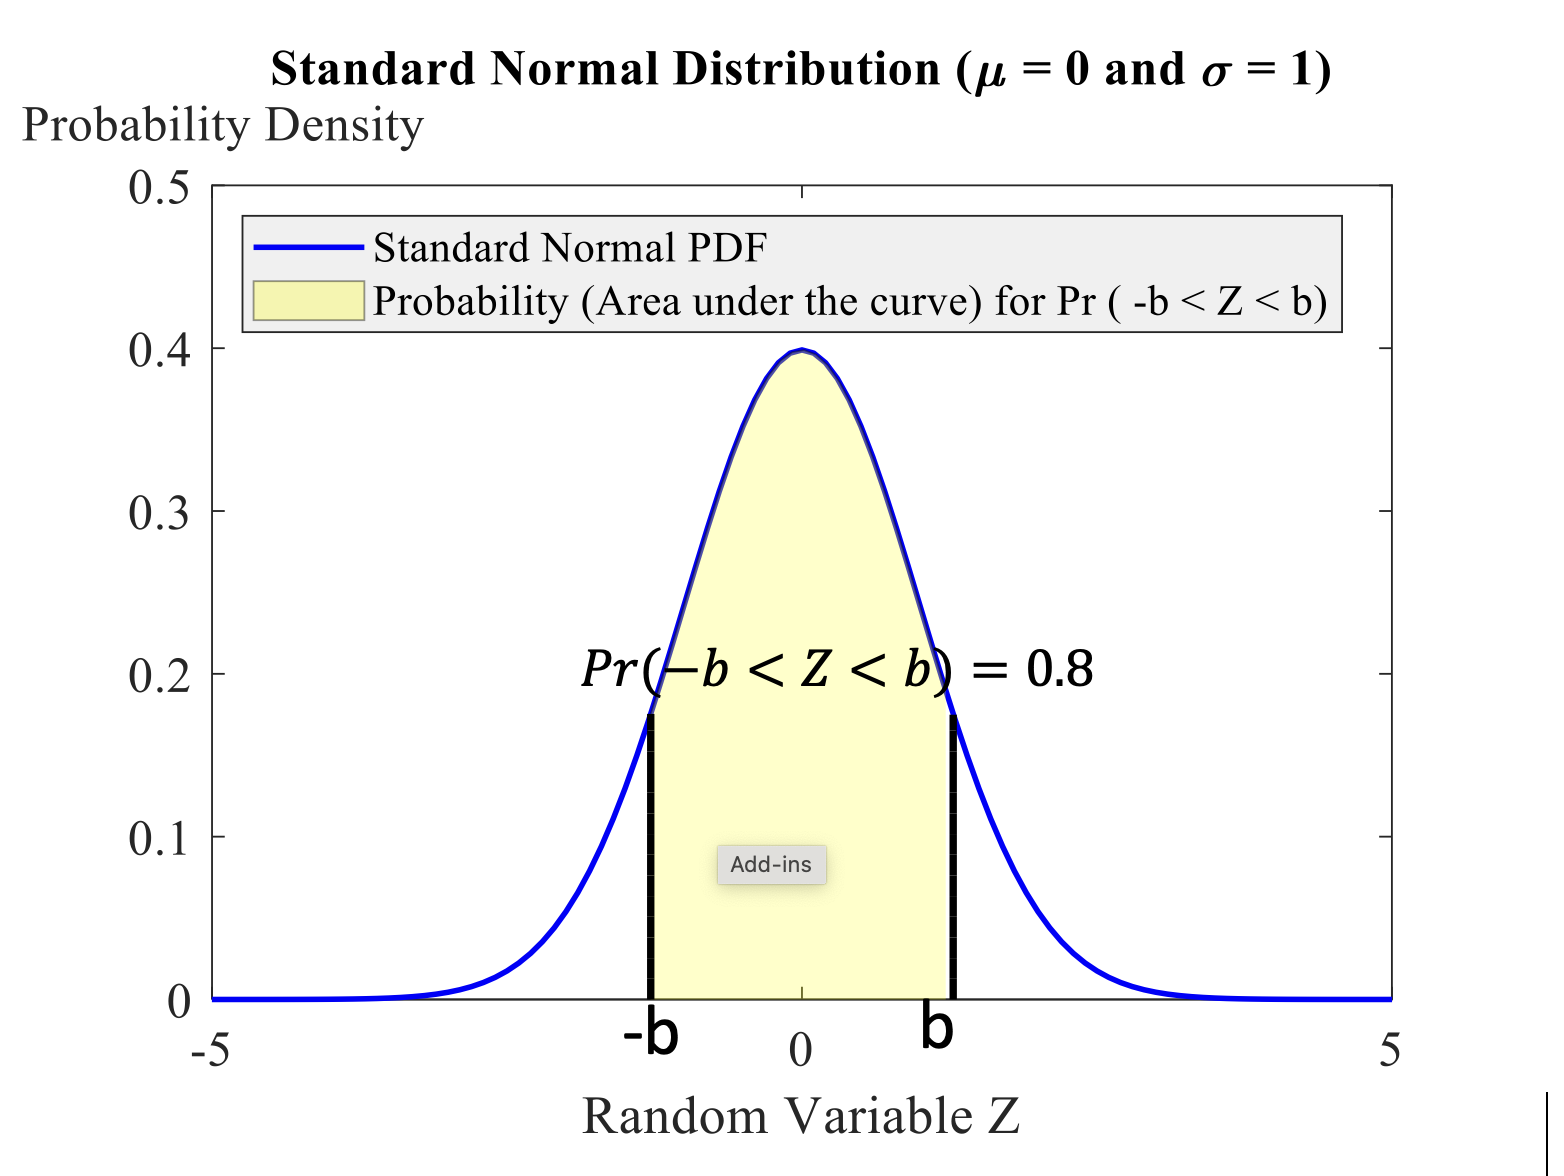
\includegraphics[width=2.82292in,height=\textheight]{Fig/q4_mu_sd_1.png}

}

\end{figure}
\end{frame}

\begin{frame}{Exercise 4 (Cont'd)}
\protect\hypertarget{exercise-4-contd-1}{}
Considering the above shape, one can argue that the white area under the
curve on the left is 10\% and the white area under the curve on the
right is also 10\%. Thus, \(\Pr(Z < b) = 0.9\)

\begin{figure}

{\centering 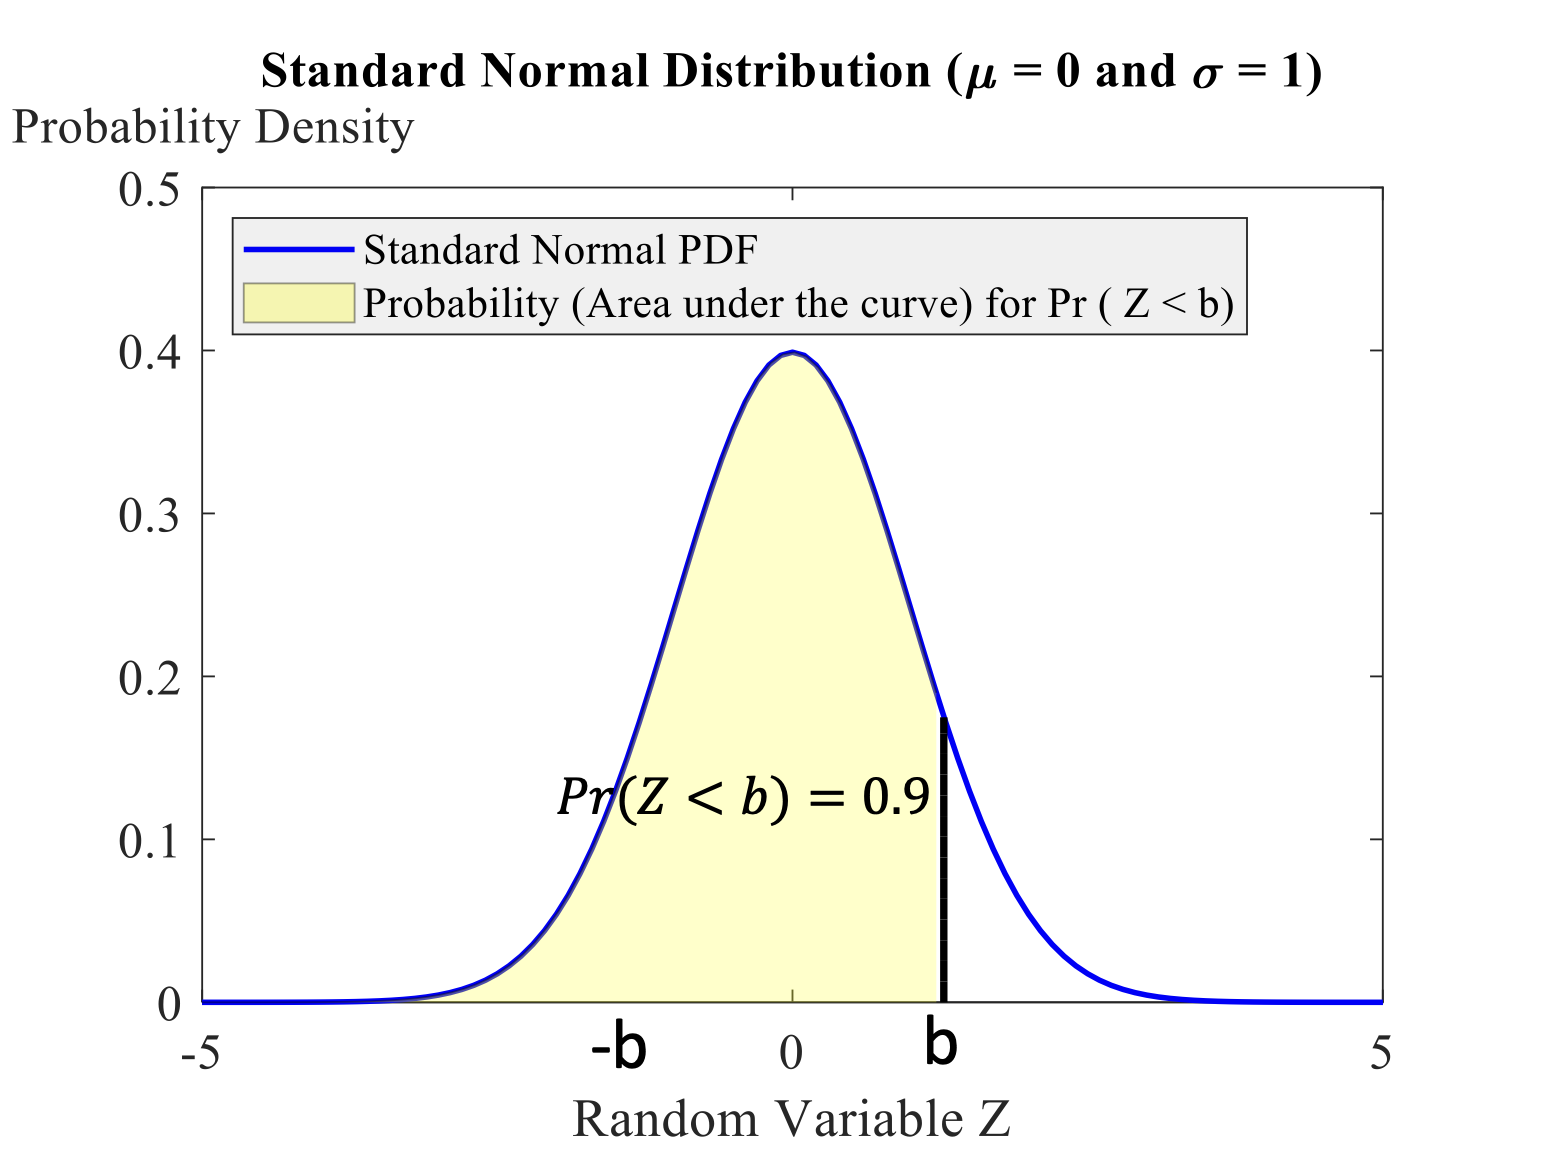
\includegraphics[width=2.82292in,height=\textheight]{Fig/q4_mu_sd_2.png}

}

\end{figure}
\end{frame}

\begin{frame}{Exercise 4 (Cont'd)}
\protect\hypertarget{exercise-4-contd-2}{}
Searching for 0.90 among the numbers (probabilities) in the \(Z\)-table,
we find that there is 0.8997 located at the intersection of 1.2 and
0.08, and 0.9015 located at the intersection of 1.2 and 0.09, which
means that \(\Pr(Z < 1.28) = 0.8997\) and \(\Pr(Z < 1.29) = 0.901\).
Therefore, \(b\) must be between 1.28 and 1.29 and should be closer to
1.28. If \(b = 1.28\), then

\[
a = 1.5 \times 1.28 = 1.92
\]
\end{frame}

\begin{frame}{Exercise 4 (Cont'd)}
\protect\hypertarget{exercise-4-contd-3}{}
\textbf{Note.}

If you want to find \(b\) more precisely, you can use interpolation
(i.e., \(b\) is the weighted average of 1.28 and 1.29). The distance
between 0.8997 and 0.9015 is 0.0018. Use 0.0018 as the weight
denominator. The distance between the probability of interest (0.90) and
0.8997 is only 0.0003. Therefore, the weight of 1.28 is \((18 - 3)/18\)
and the distance between 0.90 and 0.9015 is 0.0015, so the weight of
1.29 is \((18 - 15)/18\). As a result, a more precise \(b\) is:

\[
b = \frac{15}{18} (1.28) + \frac{3}{18} (1.29) = 1.28166
\]
\end{frame}

\begin{frame}{Exercise 5}
\protect\hypertarget{exercise-5}{}
In how many ways can I choose the following?

\begin{enumerate}
\item
  I have 6 T-shirts, and I arbitrarily choose 3 to take on holiday with
  me.

  \pause

  \textbf{A}: \vspace{-10pt}

  \[
  \begin{aligned}
  C_{x=3}^{n=6} &= \frac{n!}{x!(n - x)!} \\ 
  &= \frac{6!}{3!(6 - 3)!}  \\
  &= \frac{6 \times 5 \times 4 \times 3!}{3! \times 3!} \\
  &= 20
  \end{aligned}
  \]
\end{enumerate}
\end{frame}

\begin{frame}{Exercise 5 (Cont'd)}
\protect\hypertarget{exercise-5-contd}{}
\begin{enumerate}
\setcounter{enumi}{1}
\item
  I have a list of 10 people to call but only have time to make 3 calls
  tonight.

  \pause

  \textbf{A}: \vspace{-10pt}

  \[
  \begin{aligned}
  C_{x=3}^{n=10} &= \frac{n!}{x!(n - x)!} \\
  &= \frac{10!}{3!(10 - 3)!} \\
  &= \frac{10 \times 9 \times 8 \times 7!}{3! \times 7!} \\
  &= 120
  \end{aligned}
  \]
\end{enumerate}
\end{frame}

\begin{frame}{Exercise 5 (Cont'd)}
\protect\hypertarget{exercise-5-contd-1}{}
\begin{enumerate}
\setcounter{enumi}{2}
\item
  I have 8 friends, and I can invite just 4 to a dinner party.

  \pause

  \textbf{A}: \vspace{-20pt}

  \[
  C_{x=4}^{n=8} = \frac{n!}{x!(n - x)!} 
  = \frac{8!}{4!(8 - 4)!} 
  = \frac{8 \times 7 \times 6 \times 5 \times 4!}{4! \times 4!} 
  = 70
  \]
\item
  I have 5 male friends and 3 female friends, and I want to invite 2 men
  and 2 women to a dinner party

  \pause

  \textbf{A}: \vspace{-10pt}

  \[
  \begin{aligned}
  C_{x=2}^{n=5} \times C_{x=2}^{n=3} &= \frac{5!}{2!(5 - 2)!} \times \frac{3!}{2!(3 - 2)!} \\
  &= \frac{5 \times 4 \times 3!}{2! \times 3!} \times \frac{3 \times 2!}{2! \times 1!} \\
  &= 10 \times 3 = 30
  \end{aligned}
  \]
\end{enumerate}
\end{frame}

\begin{frame}{Exercise 6}
\protect\hypertarget{exercise-6}{}
At my university 22\% of the students enrolled are `mature'; that is,
aged 21 or over.

\begin{enumerate}
\item
  If I take a random sample of 5 students from the enrolment register
  what is the probability that exactly two students are mature?

  \pause

  \textbf{A}: We use the Binomial formula with \(n = 5\) or \(n = 7\),
  and \(p = 0.22\). \vspace{-30pt}

  \[
  \begin{aligned}
  \Pr(X = x \mid n, p) &= \frac{n!}{x!(n - x)!} p^x (1 - p)^{n - x} \\
  \Pr(X = 2 \mid 5, 0.22) &= \frac{5!}{2!(5 - 2)!} (0.22)^2 (1 - 0.22)^{5 - 2} \\ 
                          &= 0.2297
  \end{aligned}
  \]
\end{enumerate}
\end{frame}

\begin{frame}{Exercise 6 (Cont'd)}
\protect\hypertarget{exercise-6-contd}{}
\vspace{17pt}

\begin{enumerate}
\setcounter{enumi}{1}
\item
  If I take a random sample of 7 students from the enrolment register
  what is the probability that exactly two students are mature?

  \pause

  \textbf{A}: \vspace{-20pt}

  \[
  \begin{aligned}
  \Pr(X = 2 \mid 7, 0.22) &= \frac{7!}{2!(7 - 2)!} (0.22)^2 (1 - 0.22)^{7 - 2} \\
                          &= 0.2935
  \end{aligned}
  \]
\item
  If I take a random sample of 7 students from the enrolment register
  what is the probability that 2 or fewer students are mature?

  \pause

  \textbf{A}: \vspace{-20pt}

  \[
  \begin{aligned}
  \Pr(X \le 2 \mid 7, 0.22) &= \Pr(X = 0 \mid 7, 0.22) + \\
                            & \quad \; \Pr(X = 1 \mid 7, 0.22) + \\
                            & \quad \; \Pr(X = 2 \mid 7, 0.22) \\
                            &= 0.1756 + 0.3468 + 0.2935 = 0.816
  \end{aligned}
  \]
\end{enumerate}
\end{frame}

\begin{frame}{Exercise 7}
\protect\hypertarget{exercise-7}{}
On average, a bank makes 3 mistakes out of every 10,000 transactions. If
10,000 transactions are audited, what is the probability that 4 or more
mistakes are found?

\pause

\textbf{A}: \vspace{-20pt}

\[
p = \Pr(\text{success}) = \frac{3}{10,000}
\]

Because \(p\) is very small, \(n = 10,000\) is very large, and
\(\mu = np = 3 \le 7\), we can approximate the Binomial distribution by
using the Poisson distribution:

\[
\Pr(X = x \mid \mu) = \frac{\mu^x e^{-\mu}}{x!}
\]

with \(\mu = np = 3\).
\end{frame}

\begin{frame}{Exercise 7 (Cont'd)}
\protect\hypertarget{exercise-7-contd}{}
Thus, the probability of finding 4 or more mistakes would be:
\vspace{-10pt}

\[
\begin{aligned}
\Pr(X \ge 4 \mid \mu = 3) &= 1 - \Pr(X \le 3 \mid \mu = 3) \\
                          &= 1 - [\Pr(0) + \Pr(1) + \Pr(2) + \Pr(3)] \\
                          &= 1 - \left[
                                        \frac{\mu^0 e^{-3}}{0!} +
                                        \frac{\mu^1 e^{-3}}{1!} +
                                        \frac{\mu^2 e^{-3}}{2!} +
                                        \frac{\mu^3 e^{-3}}{3!}
                                        \right] \\
                          &= 1 - 0.64723188 = 0.3527681
\end{aligned}
\]

In addition, we could directly use the Binomial model with
\(n = 10,000\) and \(p = 0.0003\) to find the answer as follows:
\end{frame}

\begin{frame}{Exercise 7 (Cont'd)}
\protect\hypertarget{exercise-7-contd-1}{}
\[
\begin{aligned}
\Pr(X \ge 4 \mid n, p) &= 1 - \Pr(X \le 3 \mid n, p) \\
                       &= 1 - [\Pr(0) + \Pr(1) + \Pr(2) + \Pr(3)] \\
                       &= 1 - \Bigg[
                                \binom{10000}{0} (0.0003)^0 (1-0.0003)^{10000-0} + \\
                       \qquad         &\binom{10000}{1} (0.0003)^1 (1-0.0003)^{10000-1} + \\
                       \qquad         &\binom{10000}{2} (0.0003)^2 (1-0.0003)^{10000-2} + \\
                       \qquad         &\binom{10000}{3} (0.0003)^3 (1-0.0003)^{10000-3} \Bigg] \\
                       &= 1 - 0.6473189 = 0.35276810
\end{aligned}
\]
\end{frame}

\begin{frame}{Exercise 7 (Cont'd)}
\protect\hypertarget{exercise-7-contd-2}{}
The calculation of the above expression based on the Binomial
distribution is time-consuming. Hence, using the Poisson approximation
is more effective.
\end{frame}

\begin{frame}{Exercise 8}
\protect\hypertarget{exercise-8}{}
The length of time a doctor spends with a patient has an exponential
distribution with mean 10 minutes.

\begin{enumerate}
\item
  Assuming that the doctor does not have any free time between patients,
  how many patients, on average, does she see during an hour?
\item
  What proportion of patients spend more than 15 minutes with the
  doctor?

  \pause

  \textbf{A}: This is an Exponential distribution. One can define unit
  of time in two different ways.

  \pause

  \textbf{First}, define one unit of time as equal to one hour. Thus,
  the average of arrival rate (\(\lambda\)) is the number of times the
  doctor visits patients per hour. Since the doctor visits one patient
  per 10 minutes, he will visit 6 patients per hour. As a result,
  \(\lambda = 6\) per hour.
\end{enumerate}
\end{frame}

\begin{frame}{Exercise 8 (Cont'd)}
\protect\hypertarget{exercise-8-contd}{}
Hence, the probability of waiting time more than 15 minutes
(\(a = \frac{15}{60} = 0.25\) hour) would be:

\[
\begin{aligned}
Pr(X > a) &= e^{-\lambda a} \\
Pr(X > 0.25) &= 1 - e^{-6 \times 0.25} = 0.2231
\end{aligned}
\]
\end{frame}

\begin{frame}{Exercise 8 (Cont'd)}
\protect\hypertarget{exercise-8-contd-1}{}
\pause

\textbf{A}: \textbf{Second}, define one unit of time as equal to one
minute. Thus, the average of arrival rate (\(\lambda\)) is the number of
times the doctor visits patients per minute. Since the doctor visits one
patient per 10 minutes, he will visit 1/10 patients per minute. As a
result, \(\lambda=0.1\) per minute. Hence, the probability of waiting
time more than 15 minutes (\(a=15\) minutes) would be:

\[
\begin{aligned}
Pr(X > a) &= e^{-\lambda a} \\
Pr(X > 15) &= 1 - e^{-0.1 \times 15} = 0.2231
\end{aligned}
\]
\end{frame}



\end{document}
